\subsection{L2 TLB}
The L2 TLB is still private to the processor core.
It is neither coherent nor inclusive with the L1 I/D TLBs.
It contains a fully associative array for 2MB and 1GB super pages, and a set-associative array for 4KB pages.
The L2 TLB performs hardware page walk in case of a TLB miss.
We support RISC-V Sv39 virtual memory (i.e., 39-bit virtual address), so there are 3 steps in a page walk.
It can support multiple misses and parallel page walks.
It contains a split translation cache to reduce the penalty of page walk.
For each intermediate page-walk step, the split translation cache uses a fully associative array to cache the intermediate page-walk results.
As a result, first few steps in a page can be skipped if we hit in the split translation cache.

\subsubsection{Interface}

\begin{figure}
\begin{lstlisting}[caption={}]
interface L2Tlb;
  method Action updateVMInfo(VMInfo vmI, VMInfo vmD);
  interface L2TlbToChildren toChildren;
  interface TlbMemClient toMem;
  interface Perf#(L2TlbPerfType) perf;
endinterface
module mkL2Tlb(L2Tlb);
  // implementation
endmodule
\end{lstlisting}
\caption{Interface of L2 TLB}\label{fig:l2-tlb-ifc}
\end{figure}

Figure~\ref{fig:l2-tlb-ifc} shows the interface of the L2 TLB:
\begin{itemize}
    \item Method \code{updateVMInfo}: updates the local copy of some virtual-memory CSRs in the TLB.
    \item Subinterface \code{toChildren}: contains FIFO interfaces connected to L1 I/D TLBs.
    \item Subinterface \code{toMem}: contains FIFO interfaces connected to the coherent memory system (or more precisely, the shared L2 cache).
    \item Subinterface \code{perf}: is for querying the performance counters in the TLB.
\end{itemize}

\noindent\textbf{Conflict Matrix:}
Most methods should be conflict free.

\subsubsection{Implementation}

\begin{figure}
    \centering
    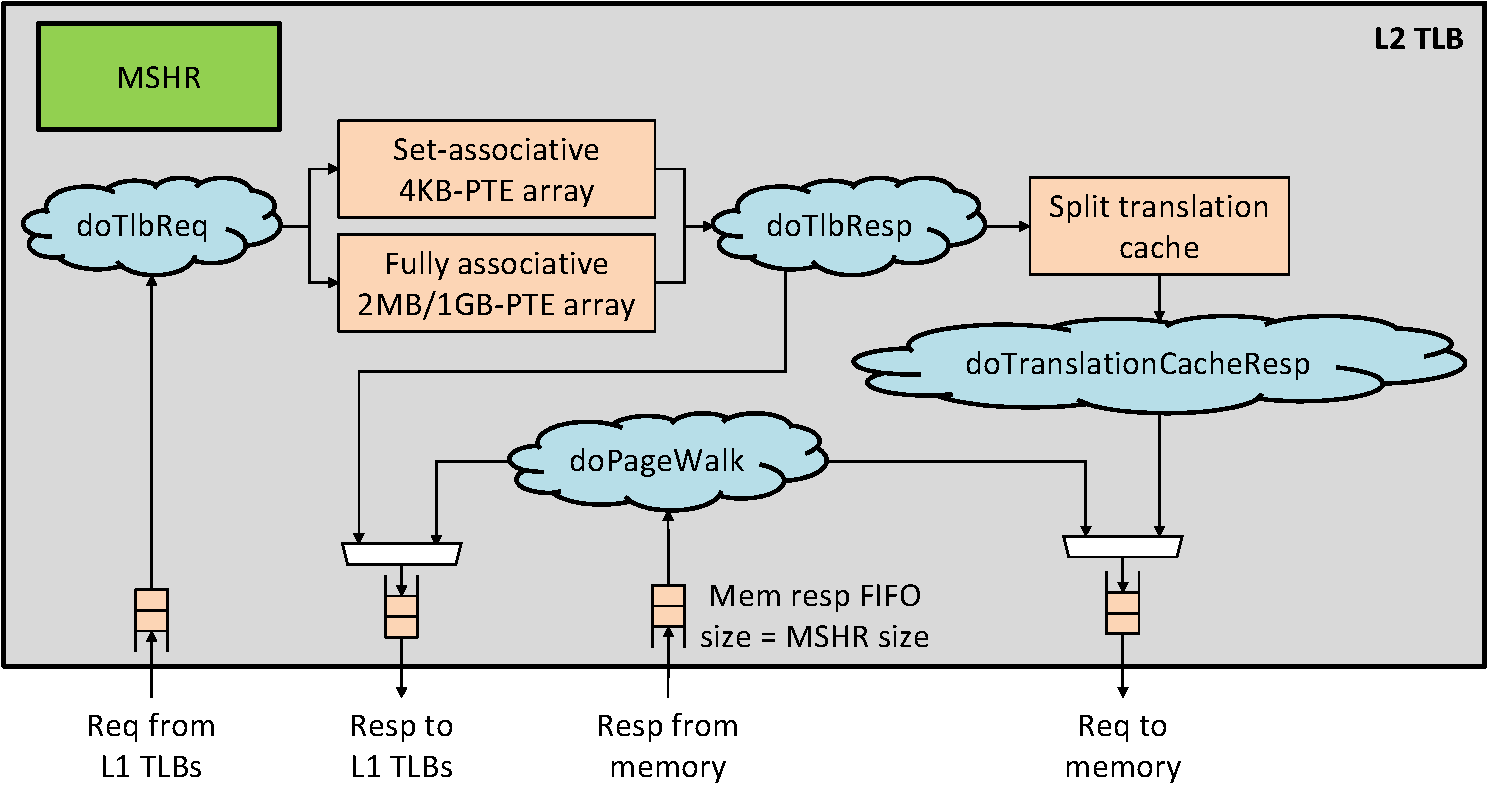
\includegraphics[width=\columnwidth]{fig/l2_tlb_crop.pdf}
    \caption{Internal implementation of L2 TLB}\label{fig:l2-tlb-impl}
\end{figure}

Figure~\ref{fig:l2-tlb-impl} shows the internal implementation of L2 TLB.
All the in-flight requests from L1 TLBs are kept in the MSHR, which is a vector of EHRs.

Every new request from the L1 TLBs is first processed by the \code{doTlbReq} rule, which allocates a new MSHR entry for the request and starts accessing the leaf-PTE arrays, i.e., both the set-associative arrays for 4KB PTEs and the fully associative array for 2MB/1GB PTEs.
Rule \code{doTlbResp} gets the response from the leaf-PTE arrays.
If we hit in the arrays, then we can directly respond the L1 TLB.
Otherwise, we continue to request the split translation cache to prepare for page walk.
Rule \code{doTranslationCacheResp} gets the response from the split translation cache, decides which steps of the page walk can be skipped, and starts the page walk by requesting the memory system.
Rule \code{doPageWalk} gets the response from the memory system, i.e., the result of the previous page walk step.
If there is a page fault or we have reached the leaf PTE, then we can respond L1 TLB.
Otherwise, we continue the page walk by requesting the memory system again.
This rule also refills the leaf-PTE arrays and the split translation cache.

We implemented an optimization to avoid duplicate requests to memory.
When we are trying to issue a request to memory for page walking, if another request has already issued the same memory request, then we do not issue a duplicate one.
The \code{doPageWalk} rule will try to satisfy as many in-flight requests as possible with a single response from memory.

\subsubsection{Source Code}
See module \code{mkL2Tlb} in \code{//procs/lib/L2Tlb.bsv}.
